\section{Introduction}

% Guttel: Matrix functions are interesting for scientific computing because they arise in explicit so- lution formulas for relevant algebraic and differential equations.
\todo[inline]{Add motivation and applications (exponential integrators, etc.)}

\subsection{Univariate Matrix Functions}
This section reviews the basic definition and properties of matrix functions discussed in detail in
\cite{higham2008functions}.
Let $A \in \mathbb{C}^{n \times n}$ have $s$ distinct eigenvalues $\{\lambda_i\}_{i=1}^{s}$. A can be
expressed in the Jordan canonical form as $A = ZJZ^{-1} = Z \diag(J_1, J_2, \dots, J_K) Z^{-1}$. Let
$ind_{\lambda_i}(A)$ denote the size of the largest Jordan block associated with $\lambda_i$. The matrix
function associated with a univariate function $f$ is defined by $f(A) := g(A)$, where $g(z)$ is the unique
Hermite interpolating polynomial of degree less than $\sum_{i=1}^{s}{ind_{\lambda_i}(A)}$. $g(z)$ which
satisfies
\begin{equation}
    \frac{\partial^j}{\partial z^j}g(\lambda_i) = \frac{\partial^j}{\partial z^j}f(\lambda_i),
    \quad \forall j \in \{0, 1, \dots, ind_{\lambda_i(A)}-1\},
    \quad \forall i \in \{1, 2, \dots, s\},
\end{equation}
assuming that all required derivatives of $f(z)$ exist.
\todo[inline]{Add the Cauchy integral definition.}

It can be shown that if $A = \diag(\lambda_i)_{i=1}^{n}$ is diagonal, we have
\begin{equation}
    \label{eq:matrixfunctiondiagonal}
    f(A) = \diag(f(\lambda_i))_{i=1}^{n}.
\end{equation}
This is simply because $A^k = \diag(\lambda_i^k)_{i=0}^{n}$ for any $k$.

For any invertible matrix $P \in \mathbb{C}^{n \times n}$, we have
\begin{equation}
    \label{eq:matrixfunctioninvertible}
    f(A) = p(A) = Pp(P^{-1}AP)P^{-1} = Pf(P^{-1}AP)P^{-1}
\end{equation}

If $A$ is diagonalizable, say $P^{-1}AP = \diag(\lambda_i)_{i=1}^{n} =: \Lambda$,
using \eqref{eq:matrixfunctioninvertible} and \eqref{eq:matrixfunctiondiagonal}
we can write
\begin{equation}
    f(A) = P f(\Lambda) P^{-1} = P \diag(f(\lambda_i))_{i=1}^{n} P^{-1}.
\end{equation}

\subsubsection*{Matrix Exponential}
The matrix function attributed to the scalar exponential function is called matrix exponential and
is defined~\cite{higham2008functions} as
\begin{equation}
    \label{eq:matrixexponentialdefinition}
    \exp(A) = \sum_{k=0}^{\infty}{\frac{1}{k!} A^k}.
\end{equation}

\todo{Summerize the properties.}
By taking the conjugate transpose of \eqref{eq:matrixexponentialdefinition}, we conclude
\begin{equation}
    \exp(A^{*}) = \exp(A)^{*}.
\end{equation}

For every $B \in \mathbb{C}^{n \times n}$ that satisfies $AB = BA$, we have
\begin{equation}
    \exp(A + B) = \exp(A) \exp(B).
\end{equation}

$\exp(A)$ is always invertible and its inverse is
\begin{equation}
    \exp(A)^{-1} = \exp(-A).
\end{equation}

The derivative of $\exp(tA)$ with respect to a scalar $t$ is given by
\begin{equation}
    \frac{\mathrm{d} \exp(tA)}{\mathrm{d} t} = A \exp(tA).
\end{equation}

The determinant of $\exp(A)$ is the exponential of the trace of $A$,
\begin{equation}
    \det(\exp(A)) = \exp(\trace(A)).
\end{equation}

\subsection{\texorpdfstring{$\varphi$}{Phi}-functions}
\todo[inline]{Add applications and motivation.}
There are a group of matrix functions called $\varphi$-functions that are essential
for exponential integrators for ordinary differential equations. Accurate and efficient
evaluation of these functions is necessary for implementation of exponential integrators.
For a scalar argument $z \in \mathbb{C}$, they are defined~\cite{higham2008functions} as
\begin{equation}
    \label{eq:scalarphifunctionsdefinition}
    \varphi_0(z) = \exp(z), \qquad
    \varphi_p(z) = \frac{1}{(p-1)!} \int_{0}^{1}{e^{(1 - \theta)z} \theta^{p-1} d\theta},
    \quad p \in \mathbb{N^*}.
\end{equation}

The $\varphi$-functions satisfy~\cite{higham2008functions} the recurrence relation
\begin{equation}
    \label{eq:scalarphifunctionsrecurrence}
    \varphi_p(z) = z^{-1} \left[ \varphi_{p-1}(z) - \frac{1}{(p-1)!} \right] ,
    \quad p \in \mathbb{N^*} \:, z \neq 0 .
\end{equation}

We can use \eqref{eq:scalarphifunctionsrecurrence} recursively as
\begin{equation*}
    \begin{aligned}
        \varphi_p(z) & = z^{-1} \varphi_{p-1}(z) - \frac{1}{(p-1)!} z^{-1} \\
        & = z^{-1} \left[ z^{-1} \varphi_{p-2}(z) - \frac{1}{(p-2)!} z^{-1} \right] - \frac{1}{(p-1)!} z^{-1} \\
        & = z^{-2} \varphi_{p-2}(z) - \frac{1}{(p-2)!} z^{-2} - \frac{1}{(p-1)!} z^{-1} \\
        & = \cdots \\
        & = z^{-p} \varphi_{0}(z) - \frac{1}{0!} z^{-p} - \frac{1}{1!} z^{-(p-1)} - \frac{1}{2!} z^{-(p-2)} - \cdots - \frac{1}{(p-1)!} z^{-1} \\
        & = z^{-p} \exp(z) - \sum_{k=0}^{p-1}{\frac{1}{k!}z^{-(p-k)}}
        \end{aligned}
\end{equation*}
to derive a closed form for $\varphi_p$:
\begin{equation}
    \label{eq:scalarphifunctionsclosedform}
    \varphi_p(z) = z^{-p} \left( \exp(z) - \sum_{k=0}^{p-1}{\frac{1}{k!}z^{k}} \right).
\end{equation}

% CHECK: What if A is singular?
For an invertible matrix $A \in \mathbb{C}^{n \times n}$, we can do the same steps and use \eqref{eq:matrixexponentialdefinition}
to get
\begin{equation}
    \label{eq:matrixphifunctionsclosedform}
    \varphi_p(A) = A^{-p} \left( \exp(A) - \sum_{k=0}^{p-1}{\frac{1}{k!}A^{k}} \right) = \sum_{k=0}^{\infty}{\frac{1}{(k+p)!} A^{k}}.
\end{equation}

\subsection{Bivariate Matrix Functions}
Let $A \in \mathbb{C}^{n \times n}$ have $s$ distinct eigenvalues $\{\lambda_i\}_{i=1}^{s}$
and $B \in \mathbb{C}^{m \times m}$ have $t$ distinct eigenvalues $\{\mu_i\}_{i=1}^{t}$.
Consider a bivariate polynomial $p(x, y) = \sum_{i=1}^{s} \sum_{j=1}^{t} p_{ij} x^i y^j$
with $p_{ij} \in \mathbb{C}$. Then $p\{A, B\}: \mathbb{C}^{m \times n} \to \mathbb{C}^{m \times n}$
is defined~\cite{kressner2014bivariate} by
\begin{equation}
    \sum_{i=1}^{s} \sum_{j=1}^{t} p_{ij} A^i C (B^\top)^j.
\end{equation}

The bivariate matrix function associated with a general bivariate scalar function $f(x, y)$ is a linear
operator on $\mathbb{C}^{n \times m}$ and is defined~\cite{kressner2014bivariate} by
$f\{A, B\} := p\{A, B\}$, where $p$ is the unique Hermite interpolating polynomial which
satisfies
\begin{equation*}
    \frac{\partial^{g+h}}{\partial x^g y^h}g(\lambda_i, \mu_j)
    = \frac{\partial^{g+h}}{\partial x^g y^h}f(\lambda_i, \mu_j),
    \quad
    \begin{matrix}
        \forall g \in \{0, 1, \dots, ind_{\lambda_i(A)}-1\},
        & \forall i \in \{1, 2, \dots, s\},
        \\
        \forall h \in \{0, 1, \dots, ind_{\mu_j(B)}-1\},
        & \forall j \in \{1, 2, \dots, t\}.
    \end{matrix}
\end{equation*}
$f$ only exists if the mixed partial derivatives in the definition exist and are continuous.

\section{Methodology}\label{sec:methods}

\subsection{Krylov Subspaces and the Arnoldi Algorithm}\label{sec:arnoldi}
\todo[inline]{Describe the Arnoldi Iteration from \cite{trefethen1997numerical}.}

\subsection{Approximation of \texorpdfstring{$\varphi$}{Phi}-functions}\label{sec:krylovmethodunivariate}

\subsubsection{Approximation}
In order to evaluate $\varphi_p(A)v$ for a matrix $A \in \mathbb{C}^{n \times n}$ and a vector $v \in \mathbb{C}$
more efficiently, we can run the Arnoldi algorithm to get an orthonormal basis $V_m \in \mathbb{C}^{n \times m}$
for the Krylov subspace of order $m$ induced by the matrix $A$ and the vector $v$:
\begin{equation}
    \label{eq:krylovsubspacedefinition}
    \mathcal{K}_m = \setspan\{v, Av, A^{2}v, \dots, A^{m-1}v \}, \quad m \leq n,
\end{equation}
and the projection of the action of $A$ on this Krylov subspace $H_m = V_m^* A V_m$. The Arnoldi factorization
reads
\begin{equation}
    \label{eq:arnoldifactorization}
    A V_m = V_m H_m + h_{m+1, m} v_{m+1} e_m^\top.
\end{equation}

\begin{lemma}
    \label{lem:krylovsubspacepowered}
    Considering the setting described above, we can write
    \begin{equation}
        A^k v = V_m H_m^k V_m^* v, \quad \forall k \in \{0, 1, \dots, m-1 \}.
    \end{equation}
\end{lemma}

\begin{proof}
    For $k=0$, it reads $V_m V_m^* v = v$ which is true because $v \in \mathcal{K}_m$ and $V_m V_m^*$
    is the projection matrix of $\mathcal{K}_m$. For $k \ge 1$, we prove by induction. Assuming that
    the lemma holds true for $k-1$, we can write
    \begin{equation*}
        A^{k} v = A A^{k-1} v = A V_m H_m^{k-1} V_m^* v.
    \end{equation*}
    Since $A^{k} v \in \mathcal{K}_m$ for all $1 \le k \le m-1$, projecting it on $\mathcal{K}_m$ will result in the same vector,
    thus
    \begin{equation*}
        A^{k} v = V_m V_m^* A^{k} v = V_m \underset{H_m}{\underbrace{V_m^* A V_m}} H_m^{k-1} V_m^* v,
    \end{equation*}
    which completes the proof.
\end{proof}

We approximate $\varphi_p(A)v$ by $\varphi_p(V_m H_m V_m^*)v$. Beacuse of orthogonality of the columns of $V_m$,
we can conclude that for any $k \in \mathbb{N}$,
\begin{equation*}
    \label{eq:reprojectionpower}
    (V_m H_m V_m^*)^{k} = V_m H_m^k V_m^*,
\end{equation*}

which could be used alongside with \eqref{eq:matrixphifunctionsclosedform} to conclude that $\varphi_p(V_m H_m V_m^*)v = V_m \varphi_p(H_m) V_m^* v$.
Because all columns of $V_m$ except the first one are orthogonal to $v$, we have $V_m^* v = \left\| v \right\|_{2} e_1$,
where $e_1$ is the first vector in the standard basis of $\mathbb{R}^n$. Putting all the pieces together, the approximation could be written as
\begin{equation}
    \label{eq:univariatephifunctionapproximation}
    \varphi_p(A)v \simeq \left\| v \right\|_{2} V_m \varphi_p(H_m) e_1.
\end{equation}
With this approximation, instead of evaluating the $\varphi$-function for a $n \times n$ matrix,
we just need to evaluate it for $H_m$ which is much smaller than $A$.

\begin{corollary}
    \label{cor:univariateerrorestimationpolynomial}
    For all $\Pi_{m-1} \ni g(z) = \sum_{k=0}^{m-1}{\alpha_k} z^k$, the approximation in \eqref{eq:univariatephifunctionapproximation} is exact;
    where $\Pi_{m-1}$ is the set of all polynomials of degree up to $m-1$.
    This can be shown using the definition of $g$ and Lemma \ref{lem:krylovsubspacepowered}:
    \begin{equation*}
        \begin{aligned}
            g(A) v & = \sum_{k=0}^{m-1}{\alpha_k A^k v}
            = \sum_{k=0}^{m-1}{\alpha_k V_m H_m^k V_m^* v}
            = V_m \underset{g(H_m)}{\underbrace{\left( \sum_{k=0}^{m-1}{\alpha_k H_m^k } \right)}}
            \underset{\left\| v \right\|_2 e_1}{\underbrace{V_m^* v}}\\
            & = \left\| v \right\|_2 V_m g(H_m) e_1.
        \end{aligned}
    \end{equation*}
\end{corollary}

\begin{lemma}
    \label{lem:hhatpowered}
    Consider a matrix $H \in \mathbb{C}^{m \times m}$.
    If we construct a matrix $\hat{H} \in \mathbb{C}^{(m+p) \times (m+p)}$ as
    \begin{equation}
        \label{eq:hhatdefinition}
        \hat{H} =
        \begin{bmatrix}
            H & e_1 & 0       \\
            0   & 0   & I_{p-1} \\
            0   & 0   & 0
        \end{bmatrix}
        \begin{matrix} m \\ p-1 \\ 1 \end{matrix}
        \begin{matrix} \quad \text{rows} \\ \quad \text{row(s)} \\ \quad \text{row} \end{matrix}
        \: ,
    \end{equation}
    with $p \ge 1$, the last column of $\hat{H}^k$, denoted by $(\hat{H}^k)_{[:, m+p]} \in \mathbb{C}^{m+p}$ takes the form
    \begin{equation*}
        \label{eq:hhatpowered}
        (\hat{H}^k)_{[:, m+p]} =
        \begin{cases}
            \begin{bmatrix} 0 \\ e_{p-k} \\ 0 \end{bmatrix}
            \begin{matrix} m \\ p-1 \\ 1 \end{matrix}
            \; \begin{matrix} \text{rows} \\ \text{row(s)} \\ \text{row} \end{matrix},
            & k \in \{ 1, 2, \dots, p-1 \}
            \\
            \begin{bmatrix} H^{k-p} e_1 \\ 0 \\ 0 \end{bmatrix}
            \begin{matrix} m \\ p-1 \\ 1 \end{matrix}
            \; \begin{matrix} \text{rows} \\ \text{rows} \\ \text{rows} \end{matrix},
            & k \ge p
        \end{cases}.
    \end{equation*}
\end{lemma}
\begin{proof}
    For $k=1$, the lemma holds by definition. For $k \ge 2$, we now show that assuming that it holds for $k-1$, it is also
    true for $k$. Since $\hat{H}^k = \hat{H} \hat{H}^{k-1}$, we can get the $m+p$\textsuperscript{th} column
    of $\hat{H}^k$, denoted by $(\hat{H}^k)_{[:, m+p]}$, by multiplying only the $m+p$\textsuperscript{th}
    column of $\hat{H}^{k-1}$. For $p-1 \ge k \ge 2$ we have
    \begin{equation*}
        \begin{aligned}
            (\hat{H}^k)_{[:, m+p]} & = \hat{H} (\hat{H}^{k-1})_{[:, m+p]} \\
            & =
            \begin{bmatrix} H & e_1 & 0\\ 0 & 0 & I_{p-1}\\ 0 & 0 & 0 \end{bmatrix}
            \begin{bmatrix} 0 \\ e_{p-k+1} \\ 0 \end{bmatrix}
            =
            \begin{bmatrix} 0 \\ e_{p-k} \\ 0 \end{bmatrix}
        \end{aligned}.
    \end{equation*}
    After each multiplication, we get the previous column of $\hat{H}$ until we reach the $m+1$\textsuperscript{th} column
    for $k=p$, $(\hat{H}^p)_{[:, m+p]} = \begin{bmatrix}e_1^\top & 0 & 0\end{bmatrix}^\top$, which is consistent with \eqref{eq:hhatpowered}.
    With this, for $k \ge p+1$ we have
    \begin{equation*}
        \begin{aligned}
            (\hat{H}^k)_{[:, m+p]} & = \hat{H} (\hat{H}^{k-1})_{[:, m+p]} \\
            & =
            \begin{bmatrix} H & e_1 & 0\\ 0 & 0 & I_{p-1}\\ 0 & 0 & 0 \end{bmatrix}
            \begin{bmatrix} H^{k-1-p} e_1 \\ 0 \\ 0 \end{bmatrix}
            =
            \begin{bmatrix} H^{k-p} e_1 \\ 0 \\ 0 \end{bmatrix}
        \end{aligned}.
    \end{equation*}
\end{proof}


To compute the approximation in \eqref{eq:univariatephifunctionapproximation}, we follow \cite{niesen2012} and read $\varphi_p(H_m) e_1$
from the first $m$ entries of the last column of $\exp(\hat{H}_m)$, with $\hat{H}_m$ defined in \eqref{eq:hhatdefinition} for $H = H_m$.
Using Lemma \ref{lem:hhatpowered} and \eqref{eq:matrixphifunctionsclosedform}, it could easily be shown that these two vectors are identical:
\begin{equation*}
    \exp(\hat{H}_m)_{[1 : m, m+p]}
    = \sum_{k=0}^{\infty}{\frac{1}{k!} (\hat{H}_m^k)_{[1 : m, m+p]}}
    = \sum_{k=p}^{\infty}{\frac{1}{k!} H_m^{k-p}e_1} = \varphi_p(H_m) e_1
\end{equation*}


\subsubsection{Error Estimation}
The method described in this section could be generalized to any function $f$ that is
analytic on a domain including the eigenvalues of $A$.

% NOTE: The result of Theorem 6.5 can be extended to general matrices by replacing [α, β] with the numerical range of A.
% For details, we refer to the seminal paper [M. Hochbruck and C. Lubich, On Krylov subspace approximations to the matrix
% exponential operator, SIAM J. Numer. Anal., 34 (1997), pp. 1911–1925].
\begin{theorem}
    \label{the:univariateerrorestimationgeneral}
    Let $A \in \mathbb{C}^{n \times n}$ be a Hermitian matrix. For a general scalar function $f: \mathbb{C} \to \mathbb{C}$ that is
    analytic on a domain $\Omega \subset \mathbb{C}$ containing the spectrum of $A$, $\Lambda(A) \subset \mathbb{R}$, the
    error of the approximation $f_m := \left\| v \right\|_{2} V_m f(H_m) e_1$ is bounded by the maximum error of the
    polynomial that approximates $f$ the best in $\Omega$:
    \begin{equation}
        \label{eq:univariateerrorestimationgeneral}
        \left\| f(A)v - f_m \right\|_2 \le 2 \left\| v \right\|_2 \min_{g \in \Pi_{m-1}} \max_{z \in \Lambda(A)} \left|f(z) - g(z) \right|
    \end{equation}
\end{theorem}
\begin{proof}
    Considering an arbitrary polynomial $g \in \Pi_{m-1}$, we define the error $e = f - g$, we use
    Corollary \ref{cor:univariateerrorestimationpolynomial}, the triangle inequality, and the orthonormality of the columns of $V_m$ to get
    \begin{equation*}
        \begin{aligned}
            \left\| f(A)v - f_m \right\|_2
                & = \left\| f(A)v \overset{zero}{\overbrace{- g(A)v + \left\| v \right\|_{2} V_m g(H_m) e_1}}
                - \left\| v \right\|_{2} V_m f(H_m) e_1 \right\|_2 \\
            & \le \left\| f(A)v - g(A)v \right\|_{2}
                + \left\| v \right\|_{2}
                \left\| V_m [g(H_m) e_1 - f(H_m) e_1] \right\|_2\\
            & \le \left\| v \right\|_2 \left( \left\| e(A) \right\|_2 + \left\| e(H_m) \right\|_2 \right)\\
            & \le 2 \left\| v \right\|_2 \max_{z \in \Lambda(A)} \left| e(z) \right|.
            \end{aligned}
    \end{equation*}
    % CHECK: How so?
    In the last step, we used that $\Lambda(H_m) \subset \Lambda(A) \subset \Omega$ holds due to eigenvalue interlacing.
\end{proof}

To specialize \autoref{the:univariateerrorestimationgeneral} to $\varphi$-functions, we follow two approaches. The
first one is using truncated Taylor series to get an approximation for the left-hand-side of
\eqref{eq:univariateerrorestimationgeneral}, which results in the following lemma.

% CHECK: Why always considering negative eigenvalues?
% NOTE: Much better estimates can be obtained, e.g., by Chebyshev expansion:
% H. Tal-Ezer, Polynomial approximation of functions of matrices and applications, J. Sci. Comput. 4 (1989), pp. 25–60
\begin{lemma}
    \label{lem:univariateerrorestimationphitaylor}
    For a phi-function $\varphi_p(z)$ defined in \eqref{eq:scalarphifunctionsclosedform} and a Hermitian matrix
    $A \in \mathbb{C}^{n \times n}$ with the spectrum $\Lambda(A) \subset [-\alpha, 0] \subset \mathbb{R}$ for $\alpha > 0$,
    the error of the approximation $\varphi_{p, m} := \left\| v \right\|_{2} V_m \varphi_p(H_m) e_1$ scales with
    $\alpha^m$:
    \begin{equation}
        \label{eq:univariateerrorestimationphitaylor}
        \left\| \varphi_p(A)v - \varphi_{p, m} \right\|_2 \le 2 \left\| v \right\|_2 \frac{\alpha^m}{(m+p)!}
    \end{equation}
\end{lemma}
\begin{proof}
    We replace the exponential in \eqref{eq:scalarphifunctionsclosedform} by its truncated Taylor expansion
    around zero and we keep the first $m+p-1$ to get
    \begin{equation*}
        \begin{aligned}
            \varphi_p(z) & = z^{-p} \left( \sum_{k=0}^{m+p-1}{\frac{1}{k!}z^k}
                + \frac{1}{(m+p)!} \abs{z}^{m+p} \exp(z') - \sum_{k=0}^{p-1}{\frac{1}{k!}z^{k}} \right)\\
            & = z^{-p} \left( \sum_{k=p}^{m+p-1}{\frac{1}{k!}z^k} + \frac{1}{(m+p)!} \abs{z}^{m+p} \exp(z') \right)\\
            & \le \sum_{k=0}^{m-1}{\frac{1}{(k+p)!}z^k} + \frac{1}{(m+p)!} \abs{z}^{m}, \quad \forall z \in \Lambda(A)
            \end{aligned}
    \end{equation*}
    where $-\alpha \le z' \le 0$. In the last step, we used $\exp(z') \le 1$ for all non-positive $z'$. By choosing $g(z) = \sum_{k=0}^{m-1}{\frac{1}{(k+p)!}z^k}$ and taking the maximum of the
    absolute value of both sides for $z \in \Lambda(A)$, we can write
    \begin{equation*}
        \max_{z \in \Lambda(A)}\left| \varphi_p(z) - g(z) \right|
        \le \frac{1}{(m+p)!} \max_{z \in \Lambda(A)}\abs{z}^{m}
        = \frac{1}{(m+p)!} \alpha^m.
    \end{equation*}
    With this, we have found a polynomial $g \in \Pi_{m-1}$ that has this error bound, so we can be sure that
    the minimum of the error bound over all polynomials in $\Pi_{m-1}$ is less than this bound. Combining this
    result with \autoref{the:univariateerrorestimationgeneral} completes the proof.
\end{proof}

Using the polynomial approximation given in \cite[Lemma A.1]{kressner2019krylov}, we can get a better error bound
for approximating $\varphi_1(A)v$.
% This approximation is only given for $p=1$, but with a minor modification in theproof, it can be shown that the same
% bound holds true for $p > 1$ as well.
The polynomial approximation states that
\begin{equation}
    \min_{g \in \Pi_{m-1}} \max_{z \in [-\alpha, 0]} \left|\varphi_1(z) - g(z) \right| \le
    \begin{cases}
        \frac{5\alpha^2}{2m^3} \exp \left( -\frac{4m^2}{5\alpha} \right) & \sqrt{\alpha} \le m \le \frac{\alpha}{2}
        \\
        \frac{32}{12m-5\alpha} \left( \frac{e \alpha}{4m+2\alpha} \right)^m & m \ge \frac{\alpha}{2}
    \end{cases}.
\end{equation}
Using this polynomial approximation error bound and combining it with \eqref{eq:univariateerrorestimationgeneral}
gives the following theorem for the Arnoldi method approximation of $\varphi_1(A)v$ for Hermitian matrices.
\begin{mdframed}
    \begin{theorem}
        \label{the:univariateerrorestimationchebyshev}
        For the phi-function $\varphi_1(z)$ defined in \eqref{eq:scalarphifunctionsclosedform} and a Hermitian matrix
        $A \in \mathbb{C}^{n \times n}$ with the spectrum $\Lambda(A) \subset [-\alpha, 0] \subset \mathbb{R}$ for $\alpha > 0$,
        the error of the approximation $\varphi_{1, m} := \left\| v \right\|_{2} V_m \varphi_1(H_m) e_1$ scales with $\alpha$ as
        \begin{equation}
            \label{eq:univariateerrorestimationphi1}
            \left\| \varphi_1(A)v - \varphi_{1, m} \right\|_2 \le
            \begin{cases}
                \left\| v \right\|_2 \frac{5\alpha^2}{m^3} \exp \left( -\frac{4m^2}{5\alpha} \right)
                & \sqrt{\alpha} \le m \le \frac{\alpha}{2}
                \\
                \left\| v \right\|_2 \frac{64}{12m-5\alpha} \left( \frac{e \alpha}{4m+2\alpha} \right)^m
                & m \ge \frac{\alpha}{2}
            \end{cases}
        \end{equation}
    \end{theorem}
\end{mdframed}

\subsection{Approximation of Bivariate Matrix Functions}\label{sec:krylovmethodbivariate}
\todo[inline]{Summerize the algorithm in \cite{kressner2019krylov}.}

\section{Implementations and Experiments}
In this section, the implementations of the methods described in \autoref{sec:methods} are presented and evaluated.
% The matrices along with their properties are listed in \autoref{tab:testmatrices}. The first three matrices are
% stiffness matrices that appear for solving the Poisson's equation with the finite difference method over a uniform
% grid. \todo{Explain more about the first three matrices.} The rest are collected from \cite{suitesparsecollection}.
In order to test the methods, we use stiffness matrices that apear in solving the Poisson's equation by the finite
difference method using a uniform mesh. The matrices are named based on the dimension of the problem and the number
of interior grid points on each dimension. For instance, \texttt{fd\_2d\_0100} denotes the matrix corresponding to
the 2D problem and using a mesh with 100 interior grid points on each dimension. These matrices are sparse, real,
symmetric, and negative definite. They are obtained by
\begin{equation*}
    \begin{aligned}
        \mathbb{R}^{n \times n} \ni fd_{1d\_n} & = (n+1)^2 K_n,\\
        \mathbb{R}^{n^2 \times n^2} \ni fd_{2d\_n} & = (n+1)^2  (I_n \otimes K_n + K_n \otimes I_n),\\
        \mathbb{R}^{n^3 \times n^3} \ni fd_{3d\_n} & = (n+1)^2  (
            I_n \otimes I_n \otimes K_n + I_n \otimes K_n \otimes I_n+ K_n \otimes I_n \otimes I_n);
        \end{aligned}
\end{equation*}
where $\otimes$ denotes the Kronicker product, $n$ is the number of interior grid points, and $K_n$ is a tridiagonal
matrix defined as
\begin{equation*}
    K_n =
    \begin{bmatrix}
        -2 & 1 & 0 & \cdots & 0 \\
        1 & -2 & 1 & \ddots & \vdots \\
        0 & 1 & -2 & \ddots & 0 \\
        \vdots & \ddots & \ddots & \ddots & 1 \\
        0 & \cdots & 0 & 1 & -2  \\
    \end{bmatrix}.
\end{equation*}

% NOTE: Smaller relgap -> worse performance of the Arnoldi method for approximating eigenvalues. Is it related?
\autoref{fig:fdndproperties} shows the smallest eigenvalues and the relative gaps of the matrices corresponding to different
number of interior grid points $n$. The magnitude of the smallest eigenvalue scales with $(n+1)^2$ and the relative gap
decreases rapidely when $n$ grows. When computing $\varphi_p(tA)$, the step size is considered as $t = 1 / (n + 1)$, so that
the magnitude of the smallest eigenvalue of the matrix $tA$ scales with $(n+1)$.

\todo{Add definition of relgap}
\begin{figure}[h!]
    \centering
    \begin{subfigure}[b]{0.45\textwidth}
        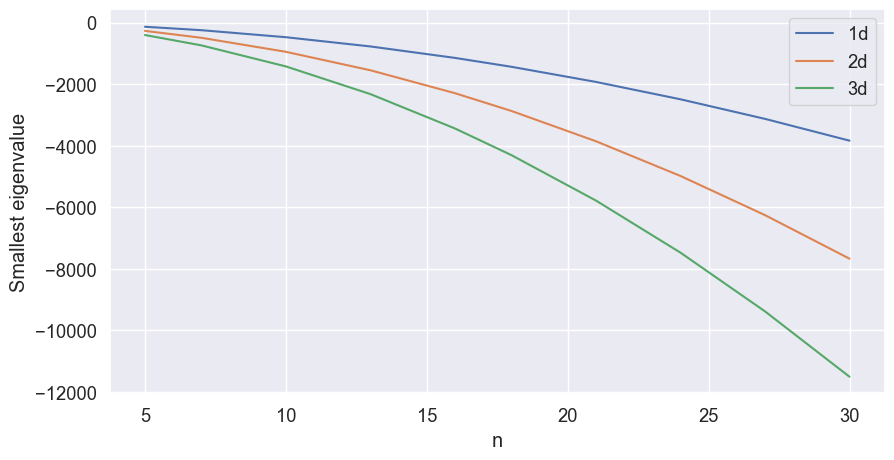
\includegraphics[width=\textwidth]{img/fd_nd_eigvals.png}
        \caption{Smallest eigenvalues.}
        \label{fig:fdndeigvals}
    \end{subfigure}
    \hfill
    \begin{subfigure}[b]{0.45\textwidth}
        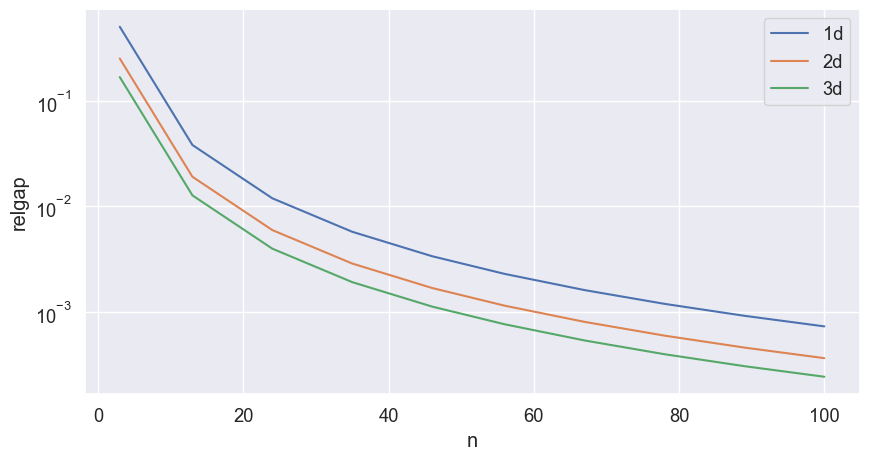
\includegraphics[width=\textwidth]{img/fd_nd_relgaps.png}
        \caption{Relative gaps.}
        \label{fig:fdndrelgaps}
    \end{subfigure}
    \caption{Smallest eigenvalues and relative gaps of the test matrices for different number of grid points.}
    \label{fig:fdndproperties}
\end{figure}


% NOTE: Old table of test matrices
\begin{comment}
\begin{table}[h!]
    \centering
    \caption{
        Properties of the test matrices. The last column is the interval that includes the eigenvalues of the matrix,
        reported only if the matrix is Hermitian.
        }
    \label{tab:testmatrices}
    \begin{tabular}[h!]{|c||c|c|c|c|c|c|}
        \hline
        Name & Size & Density & Hermitian & \makecell{Full\\numerical\\rank} & \makecell{Condition\\number} & $\Omega \subset \mathbb{R}$ \\
        \hline
        \texttt{fd\_1d} & 4096 & 0.0007 & \checkmark & \checkmark & 6.80e+06 & $[-4, 0]$ \\
        \hline
        \texttt{fd\_2d} & 4096 & 0.0012 & \checkmark & \checkmark & 1.71e+03 & $[-8, 0]$ \\
        \hline
        \texttt{fd\_3d} & 4096 & 0.0012 & \checkmark & \checkmark & 1.16e+02 & $[-8, 0]$ \\
        \hline
        \texttt{orani678} & 2529 & 0.0141 & \texttimes & \checkmark & 9.58e+03 & - \\
        \hline
        \texttt{bcspwr10} & 5300 & 0.0008 & \checkmark & \texttimes & 1.58e+17 & $[-3, 7]$ \\
        \hline
        \texttt{gr\_30\_30} & 900 & 0.0096 & \checkmark & \checkmark & 1.95e+02 & $[0, 12]$ \\
        \hline
        \texttt{helm2d03} & 392257 & < 0.0001 & \checkmark & \checkmark & ? & $[0, 11]$ \\
        \hline
    \end{tabular}
\end{table}
\end{comment}

% NOTE: Daniel said they are a bit unrelated to the topic
\begin{comment}
\begin{figure}[h!]
    \centering
    \begin{subfigure}[b]{0.45\textwidth}
        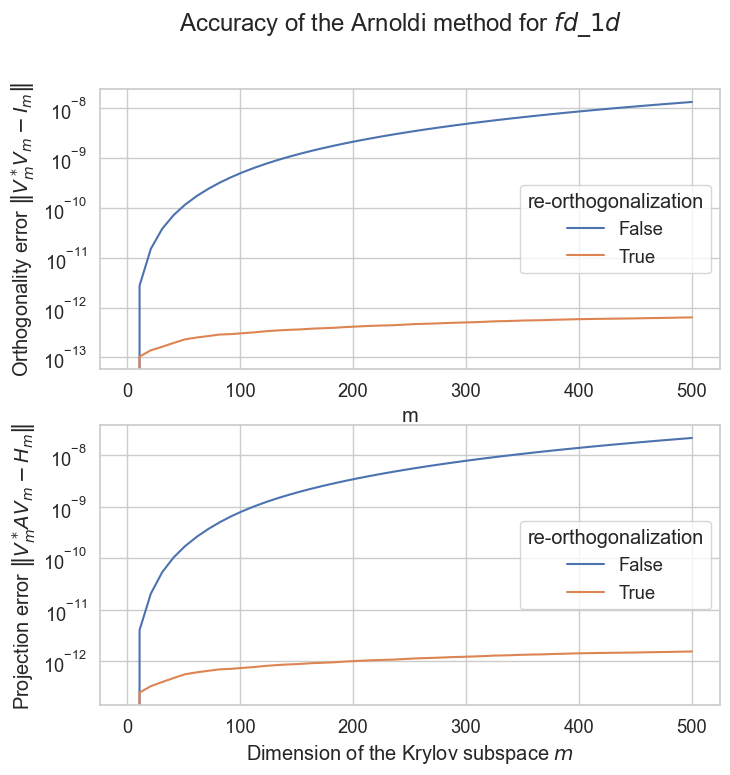
\includegraphics[width=\textwidth]{img/arnoldi/fd_1d.png}
        \caption{\texttt{fd\_1d}.}
    \end{subfigure}
    \hfill
    \begin{subfigure}[b]{0.45\textwidth}
        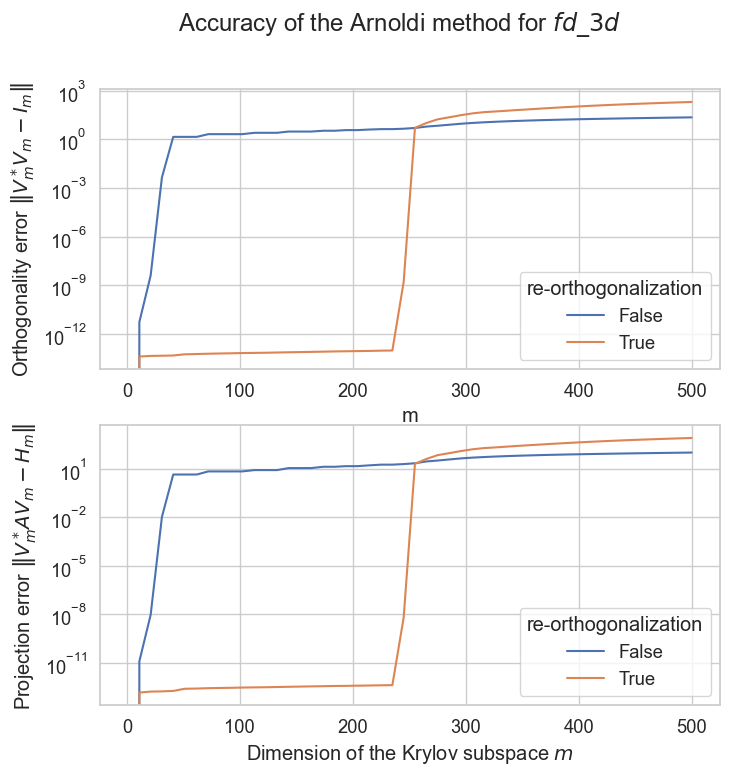
\includegraphics[width=\textwidth]{img/arnoldi/fd_3d.png}
        \caption{\texttt{fd\_3d}.}
    \end{subfigure}
    \vfill
    \begin{subfigure}[b]{0.45\textwidth}
        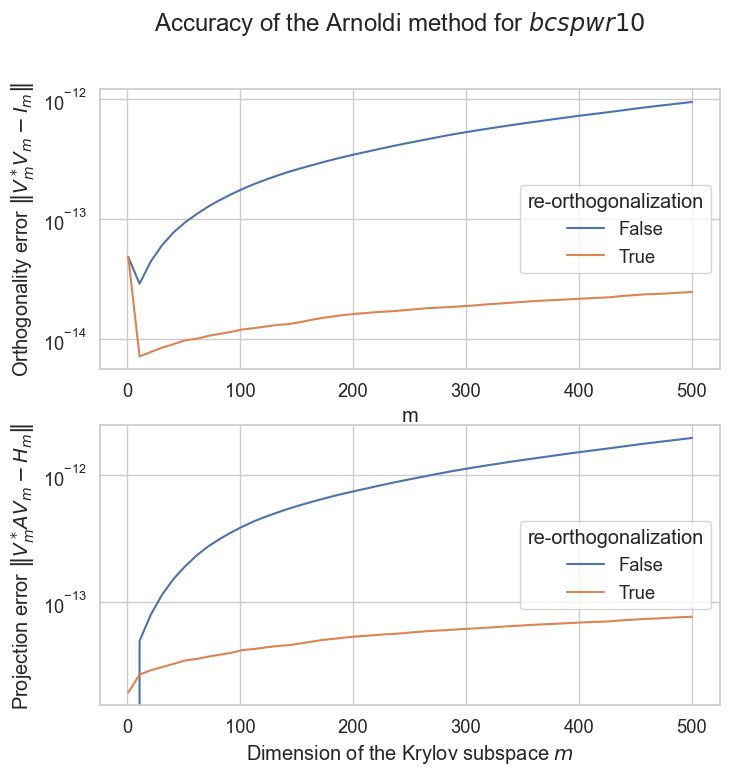
\includegraphics[width=\textwidth]{img/arnoldi/bcspwr10.png}
        \caption{\texttt{bcspwr10}.}
    \end{subfigure}
    \hfill
    \begin{subfigure}[b]{0.45\textwidth}
        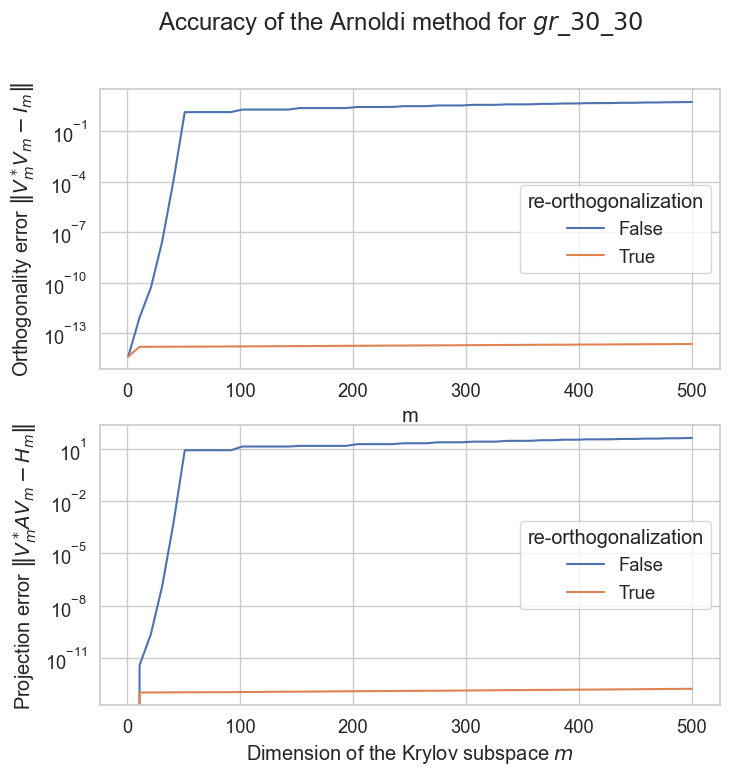
\includegraphics[width=\textwidth]{img/arnoldi/gr_30_30.png}
        \caption{\texttt{gr\_30\_30}.}
    \end{subfigure}
    \caption{Evaluation of the implemented Arnoldi algorithm with different matrices.}
    \label{fig:arnoldievaluation}
\end{figure}

\subsection{Arnoldi Algorithm}
The Arnoldi Algorithm described in \autoref{sec:arnoldi} is implemented as in (\autoref{lst:arnoldialgorithm}).
In order to make sure that the implementation is working well, it is applied on the test matrices with different
dimensions of the Krylov subspace $m$. Each experiment is done once with the re-orthogonalization steps and once
without it. To evaluate the quality of the outputs, we measure two residuals: 1. the deviation of $V_m^* V_m$ from the
identity matrix $I_m$ to check the orthogonality of the basis vectors; 2. the deviation of the projection of the
action of $A$ on the Krylov subspace given by $V_m^* A V_m$ from the output $H_m$. For both measures, we report the
spectral norm of the matrices.

Figure~\ref{fig:arnoldievaluation} depicts the results for four matrices. First of all, we can see that the accuracy
of the method always deteriorates for higher dimensions of Krylov subspace. However, for almost all the cases, the
errors are in an acceptable range for up to $m=500$, if re-orthogonalization is applied. This is not the case for the
matrix \texttt{fd\_3d}, where the errors explode after around $m=200$. Furthermore, we can see that re-orthogonalization
always improves the accuracy of the method up to several orders of magnitude. By looking at the plots corresponding to \texttt{gr\_30\_30}, we can see that without re-orthogonalization,
the performance of the method is not acceptable even for small $m$'s.
\end{comment}

\begin{figure}[h!]
    \centering
    \begin{subfigure}[b]{0.45\textwidth}
        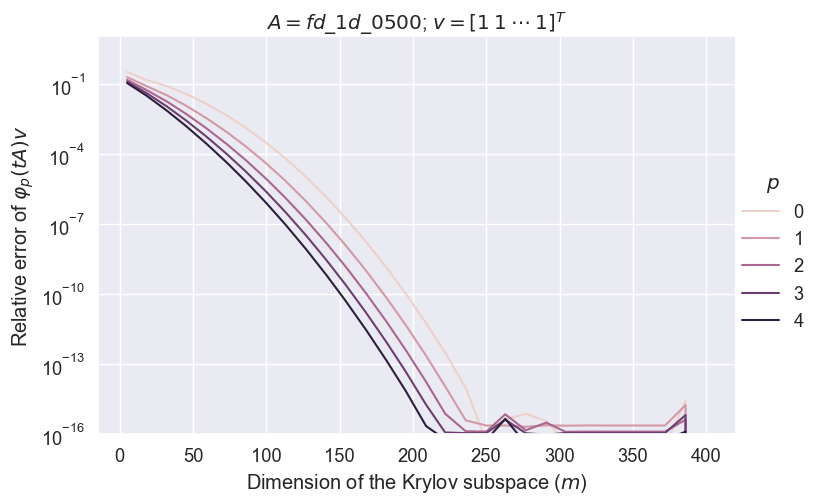
\includegraphics[width=\textwidth]{img/krylovunivariate/fd_1d_0500.png}
        \caption{\texttt{fd\_1d\_0500}.}
    \end{subfigure}
    \hfill
    \begin{subfigure}[b]{0.45\textwidth}
        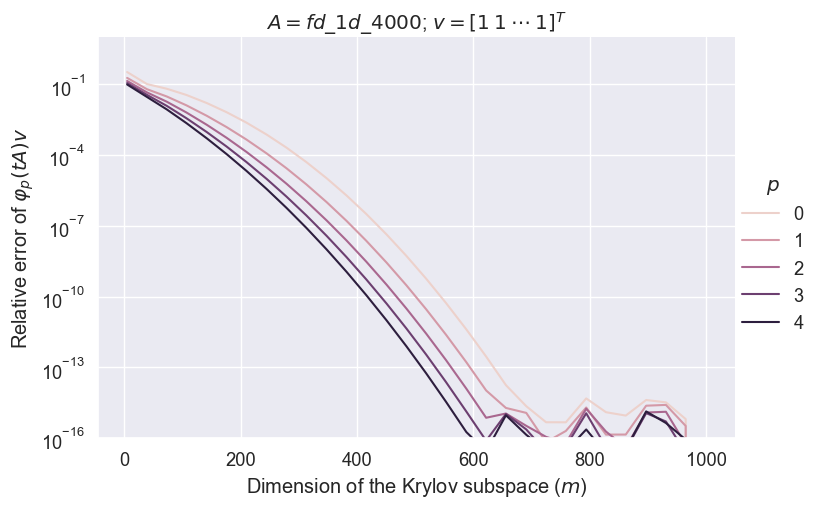
\includegraphics[width=\textwidth]{img/krylovunivariate/fd_1d_4000.png}
        \caption{\texttt{fd\_1d\_4000}.}
    \end{subfigure}
    \vfill
    \begin{subfigure}[b]{0.45\textwidth}
        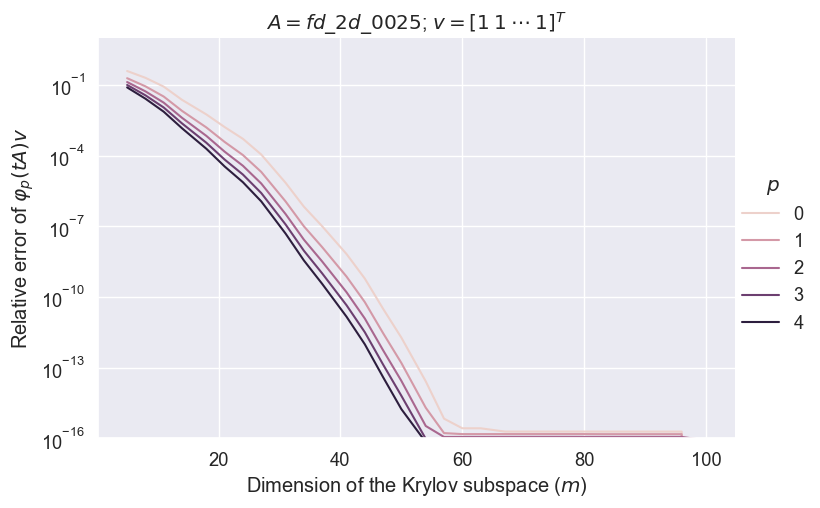
\includegraphics[width=\textwidth]{img/krylovunivariate/fd_2d_0025.png}
        \caption{\texttt{fd\_2d\_0025}.}
    \end{subfigure}
    \hfill
    \begin{subfigure}[b]{0.45\textwidth}
        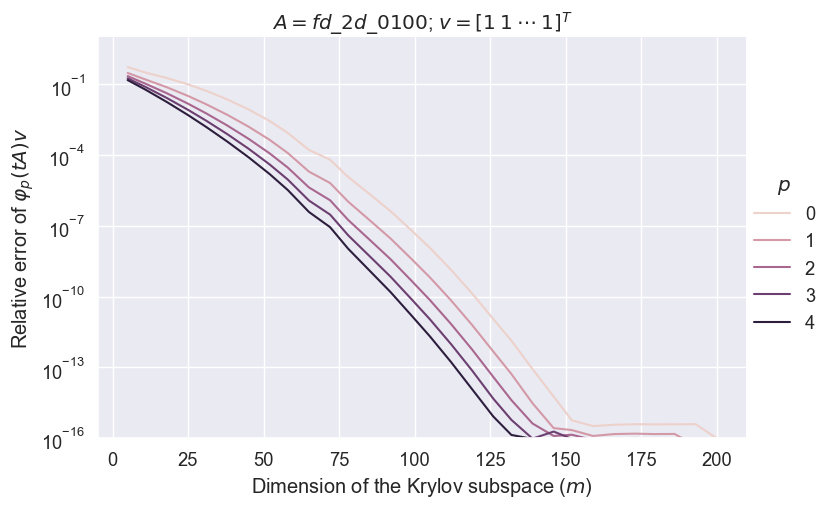
\includegraphics[width=\textwidth]{img/krylovunivariate/fd_2d_0100.png}
        \caption{\texttt{fd\_2d\_0100}.}
    \end{subfigure}

    \caption{Convergence of the apprixmation \eqref{eq:univariatephifunctionapproximation} for different matrices.}
    \label{fig:krylovmethodunivariateevaluation}
\end{figure}


\subsection{Approximation of Phi-functions}
The method described in \autoref{sec:krylovmethodunivariate} is implemented and its approximations have been evaluated
for different matrices. The implementation is presented in \autoref{lst:krylovmethodunivariate}.
For computing $\exp(\hat{H}_m)$, the \texttt{scipy.linalg.expm} function from the the SciPy library~\cite{SciPy2020}
is used which implements a Pade approximation with a variable order that is decided based on the array data.
In order to validate the implementation, we use an implementation of \eqref{eq:matrixphifunctionsclosedform}, presented in
\autoref{lst:matrixphifunctionsclosedform}, and we look at the relative error of the results from the Krylov subspace
method of dimension $m$, denoted by $\varphi_p^{(m)}(tA)v$, against the vectors computed by \eqref{eq:matrixphifunctionsclosedform},
denoted by $\varphi_p(tA)v$, for different matrices and for small $p$'s. The relative error is computed as:
\begin{equation*}
    \frac{\left\| \varphi_p^{(m)}(tA)v - \varphi_p(tA)v \right\|_2}{\left\| \varphi_p(tA)v\right\|_2}.
\end{equation*}
After the implementation is validated, we take the approximations with $m=m^*$ as reference and we compute
\begin{equation*}
    \frac{\left\| \varphi_p^{(m)}(tA)v - \varphi_p^{(m^*)}(tA)v \right\|_2}{\left\| \varphi_p^{(m^*)}(tA)v\right\|_2}
\end{equation*}
for $0 \le p \le 4$. For each matrix, $m^*$ is picked large enough so that the method converges before $m=m^*$.
The convergence plots are illustrated in \autoref{fig:krylovmethodunivariateevaluation}.
For all the test matrices, the approximations are carried out for a vector of ones of a suitable size.

\begin{remark}
    The reason that the relative errors are not reported against the results of the implementation of
    \eqref{eq:matrixphifunctionsclosedform} is that this implementation seems to work poorly as $p$ increases.
    One reason could be that we need to compute the inverse of $A^p$ for this method. Although computation of the
    inverse is avoided by solving the corresponding system of equations instead, it can still perform poorly because
    the condition number of $A^p$ grows as $p$ is increased. This hypothesis is supported by
    \autoref{fig:krylovmethodunivariateevaluationrecursive} where the convergence plots are computed against this implementation
    for two matrices. We can see that as $p$ is increased, the minimum error that is reached by the approximation gets worse.
    This shows that the approximation is performing better than the implementation of \eqref{eq:matrixphifunctionsclosedform}.
    Furthermore, this pattern is more severe for the matrix \texttt{fd\_1d\_0500} which has a bigger condition number
    than \texttt{fd\_2d\_0100}.
\end{remark}

\begin{figure}[h!]
    \centering
    \begin{subfigure}[b]{0.45\textwidth}
        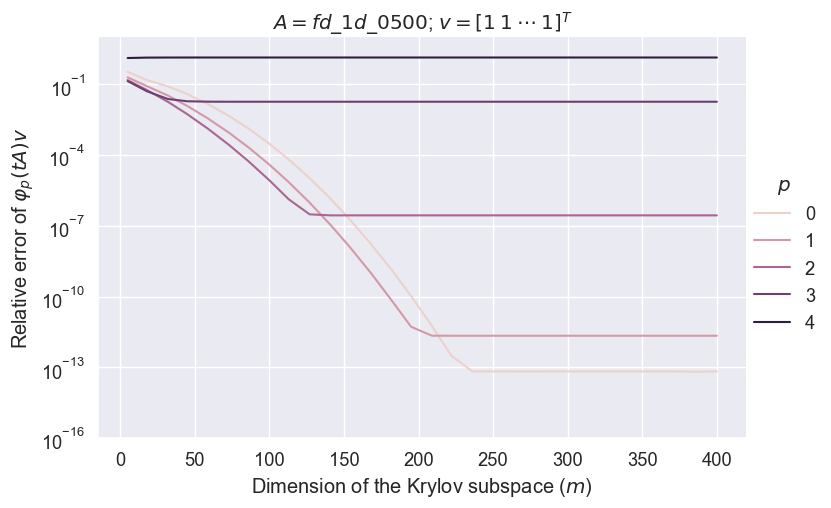
\includegraphics[width=\textwidth]{img/krylovunivariate/fd_1d_0500_recursive.png}
        \caption{\texttt{fd\_1d\_0500}.}
    \end{subfigure}
    \hfill
    \begin{subfigure}[b]{0.45\textwidth}
        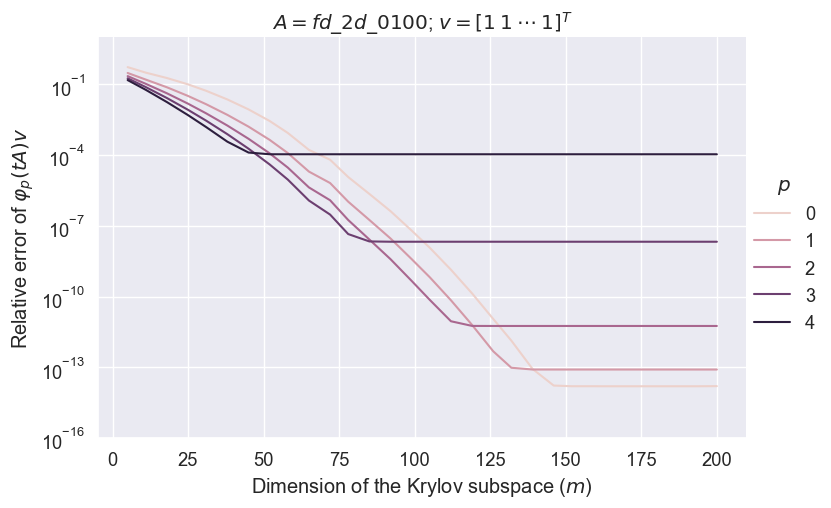
\includegraphics[width=\textwidth]{img/krylovunivariate/fd_2d_0100_recursive.png}
        \caption{\texttt{fd\_2d\_0100}.}
    \end{subfigure}
    \caption{Convergence of the apprixmation \eqref{eq:univariatephifunctionapproximation} against
    the implementation of \eqref{eq:matrixphifunctionsclosedform} for matrices with mild condition numbers.}
    \label{fig:krylovmethodunivariateevaluationrecursive}
\end{figure}

\begin{figure}[h!]
    \centering
    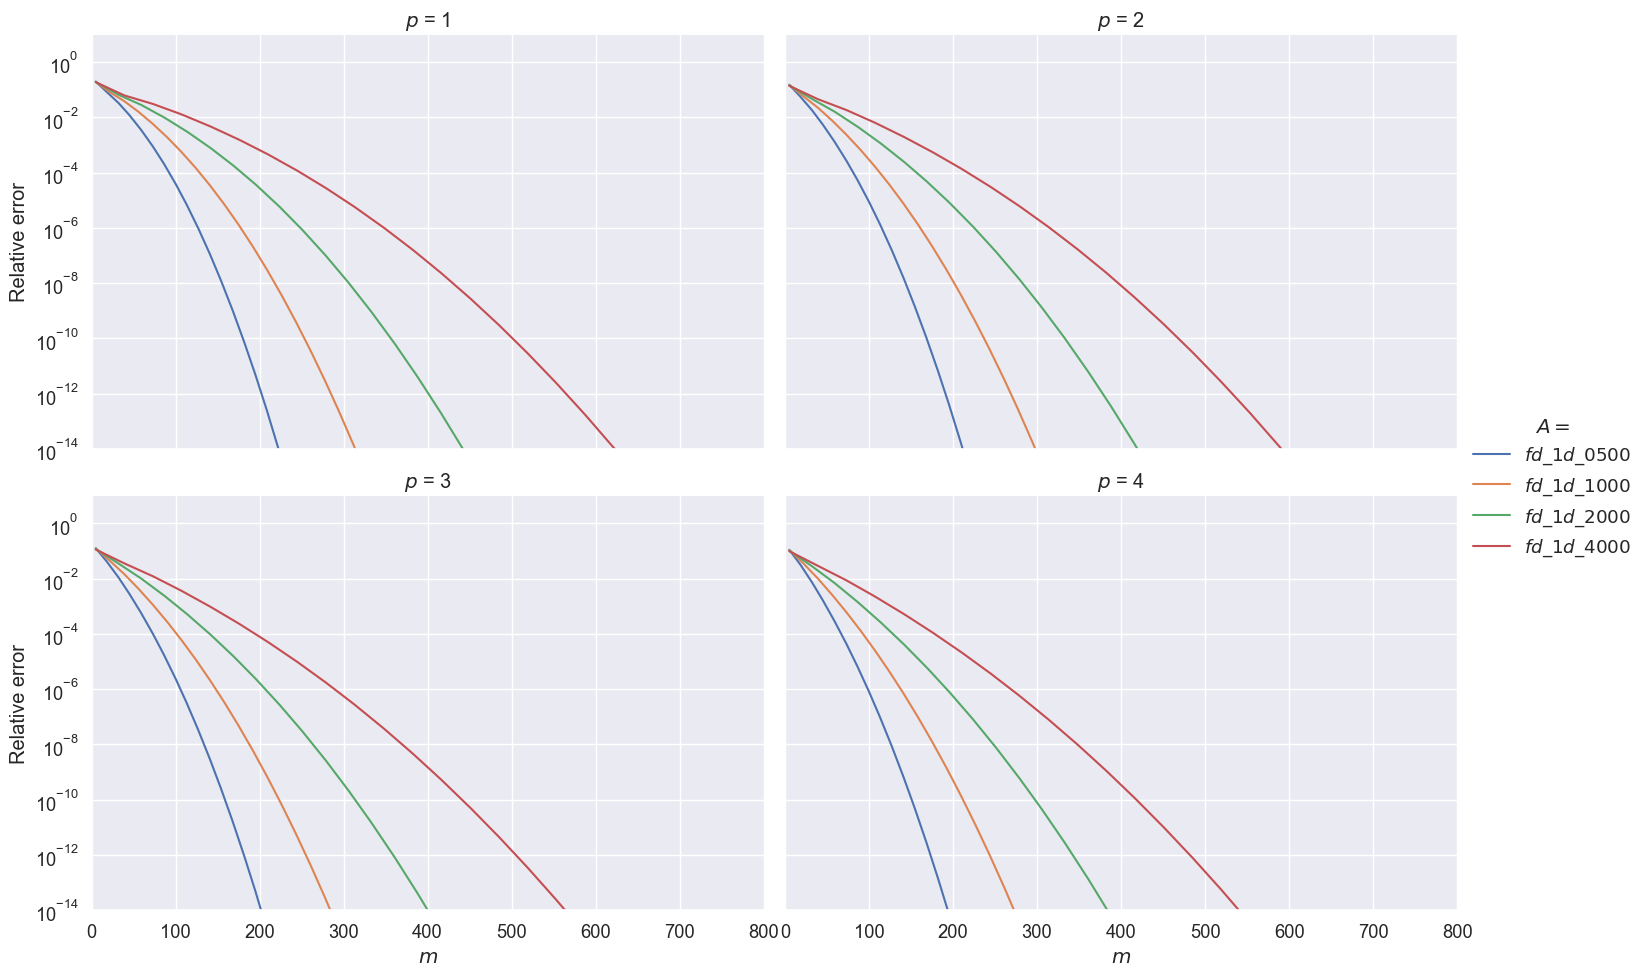
\includegraphics[width=.9\textwidth]{img/krylovunivariate/compare_fd_1d_n.png}
    \caption{Comparison of the convergence rate of the apprixmation \eqref{eq:univariatephifunctionapproximation} for different matrices.}
    \label{fig:krylovmethodunivariatecomparespectrums}
\end{figure}

The error estimates given in Lemma \ref{lem:univariateerrorestimationphitaylor} and \autoref{the:univariateerrorestimationchebyshev}
show that the eigenvalues of the matrix change the rate of convergence of the method. They also show that the starting error
decreases for larger $p$'s. It could be confirmed by looking at the plots in \autoref{fig:krylovmethodunivariateevaluation} that
the second interpretation is consistent with the numerical results. \autoref{fig:krylovmethodunivariatecomparespectrums} emphasizes
on the first interpretation by comparing the convergence of matrices with different spectrums. We can see that the method converges
faster when the smallest eigenvalue of the matrix is smaller in magnitude and this pattern is consistent for different $p$'s.

\begin{figure}[h!]
    \centering
    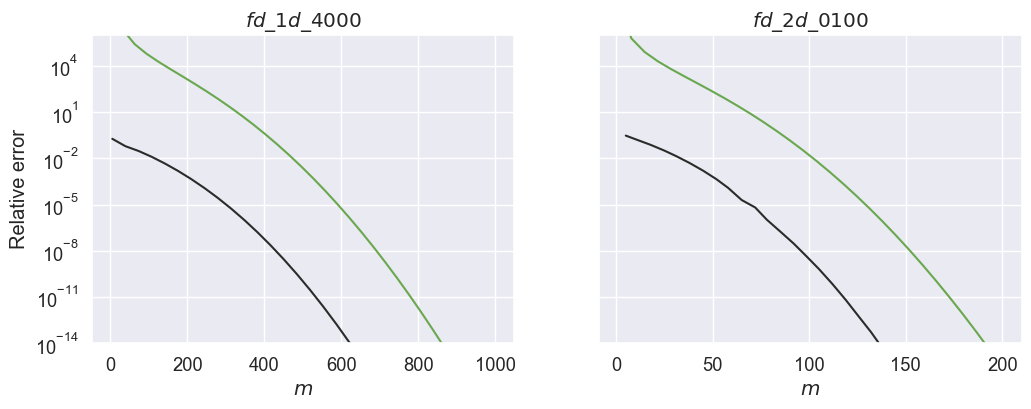
\includegraphics[width=.9\textwidth]{img/krylovunivariate/compare_errorbounds.png}
    \caption{
        Convergence of two matrices against their the theoretical error estimates;
        black: numerical results,
        green: theoretical error estimate of \autoref{the:univariateerrorestimationchebyshev}.
        }
    \label{fig:krylovmethodunivariatecompareerrorestimations}
\end{figure}

\autoref{fig:krylovmethodunivariatecompareerrorestimations} compares the theoretical error estimate with the numerical
results for two matrices. We can see that the numerical rate of convergence is consistent with the one from the theoretical
error estimate.
